% IEEE Paper Template for A4 Page Size (V1)
% Sample Conference Paper using IEEE LaTeX style file for A4 pagesize.
% Copyright (C) 2006-2008 Causal Productions Pty Ltd.
% Permission is granted to distribute and revise this file provided that
% this header remains intact.
%
% REVISION HISTORY
% 20080211 changed some space characters in the title-author block
%
\documentclass[11pt,conference,a4paper]{IEEEtran}
\usepackage{times,amsmath,epsfig}

\usepackage{multirow}
\usepackage{listings}
\usepackage{color}

%
% Kommandos für das Zitieren.
%
\newcommand{\zitiereSeite}[2]{\cite[][S.#2]{#1}}
\newcommand{\zitiereKapitel}[2]{\cite[][Kap.#2]{#1}}
\newcommand{\zitiere}[1]{\cite[]{#1}}

\newcommand{\vergleiche}[2]{(nach \cite[][S.#2]{#1})}

\newcommand{\sieheSeite}[2]{(siehe \cite[][S.#2]{#1})}
\newcommand{\sieheKapitel}[2]{(siehe \cite[][Kap.#2]{#1})}
\newcommand{\siehe}[1]{(siehe \cite{#1})}
%
% Kurzkommandos für Abbildungen, sowohl zum Referenzieren als auch zum Einfügen
%

%
% Kommandos für Textersetzungen, Fett, Kursiv, Mehrzeilig,...
%
\newcommand{\dbcommand}[1]{\textit{#1}}
\newcommand{\dbfile}[1]{\textit{#1}}
\newcommand{\dbname}[1]{\textbf{#1}}

\newcommand{\klasse}[1]{\textbf{#1}}
\newcommand{\member}[1]{\textit{#1}}
\newcommand{\funktion}[1]{\texttt{#1}}

\newcommand{\controller}[1]{\textbf{#1}}
\newcommand{\resource}[1]{\textit{#1}}


\definecolor{dkgreen}{rgb}{0,0.6,0}
\definecolor{gray}{rgb}{0.5,0.5,0.5}
\definecolor{mauve}{rgb}{0.58,0,0.82}

\lstset{frame=tb,
  language=Java,
  aboveskip=3mm,
  belowskip=3mm,
  basicstyle={\small\ttfamily},
  numberstyle=\tiny\color{gray},
  keywordstyle=\color{blue},
  commentstyle=\color{dkgreen},
  stringstyle=\color{mauve},
  captionpos=b
}
\renewcommand{\lstlistingname}{Ausschnitt}
\renewcommand{\lstlistlistingname}{List von \lstlistingname en}
%
\title{Dalvik VM}
%
\author{%
% author names are typeset in 11pt, which is the default size in the author block
{Reinhard Penn, Sebastian Ratzenboeck}%
% add some space between author names and affils
\vspace{1.6mm}\\
\fontsize{10}{10}\selectfont\itshape
% 20080211 CAUSAL PRODUCTIONS
% separate superscript on following line from affiliation using narrow space
Embedded Systems Design, FH Oberösterreich\\
Campus Hagenberg\\
\fontsize{9}{9}\selectfont\ttfamily\upshape
%
% 20080211 CAUSAL PRODUCTIONS
% in the following email addresses, separate the superscript from the email address
% using a narrow space \,
% the reason is that Acrobat Reader has an option to auto-detect urls and email
% addresses, and make them 'hot'. Without a narrow space, the superscript is included
% in the email address and corrupts it.
% Also, removed ~ from pre-superscript since it does not seem to serve any purpose
$^{1}$\,S1410567017@students.fh-hagenberg.at\\
$^{3}$\,S1419002063@students.fh-hagenberg.at%
% add some space between email and affil
\vspace{1.2mm}\\
}
%
\begin{document}
\maketitle
%
\begin{abstract}
This paper is about the Dalvik Virtual Machine. The goals are to give a short overview on the Dalvik VM and its function. Furthermore the \member{.dex} file format will be explained. In the end a comparison between the Dalvik VM and the newer Android Runtime will take place.
\end{abstract}

%
\begin{figure}
\centering

\includegraphics[width=0.25\textwidth]{AndroidRobot}
\caption{Android Logo\cite{6}}
\label{fig:AndroidRobot}
\end{figure}

\section{Allgemeines\cite{3}}
Bei Dalvik handelt es sich um eine Open Source Software die von Dan Bornstein entwickelt wurde. Benannt ist sie nach einem Fischerdorf in Eyjafjoerour, Island. Veroeffentlicht wurde die Software unter Apache License 2.0. Die Ausfuehrung findet auf einem Linux Kernel statt.
\\
\\
Verwendung findet Dalvik in Googles Betriebssystem Android. Einsatz findet Dalvik hierbei als virtuelle Maschine. Der Hauptverwendungsbereich liegt im Mobilbereich, wie zum Beispiel bei Smartphones, Tablets und seit neuestem auch bei Smart Tvs und Wearables, wie Smartwatches.


\section{Architektur\cite{2}}
In diesem Kapitel wird die Architektur der Dalvik Virtual Machine erklaert. Besonderes Augenmerk wird hierbei auf den Aufbau der \member{.dex} Datei gelegt.


\subsection{Funktion}
In Abbildung 2 ist die allgemeine Architektur von Android zu sehen. In ihr sieht man, dass die Dalvik Virtual Machine Teil der Android Runtime ist. In Android bekommt jeder Prozess seine eigene virtuelle Maschine, bei dieser handelt es sich um eine Dalvik VM. Sie aehnelt teilweise einer Java VM. Ein bedeutender Unterschied ist allerdings, dass eine Java VM stapelbasiert und eine Dalvik VM registerbasiert arbeitet. Diese registerbasierte Arbeitsweise lehnt sich an moderne Prozessorarchitekturen an. Sie verarbeitet Registermaschinencode, dadurch wird die Dalivk VM schneller als die Java VM und ist ressourcenschonender.
\\
\begin{figure*}
\centering
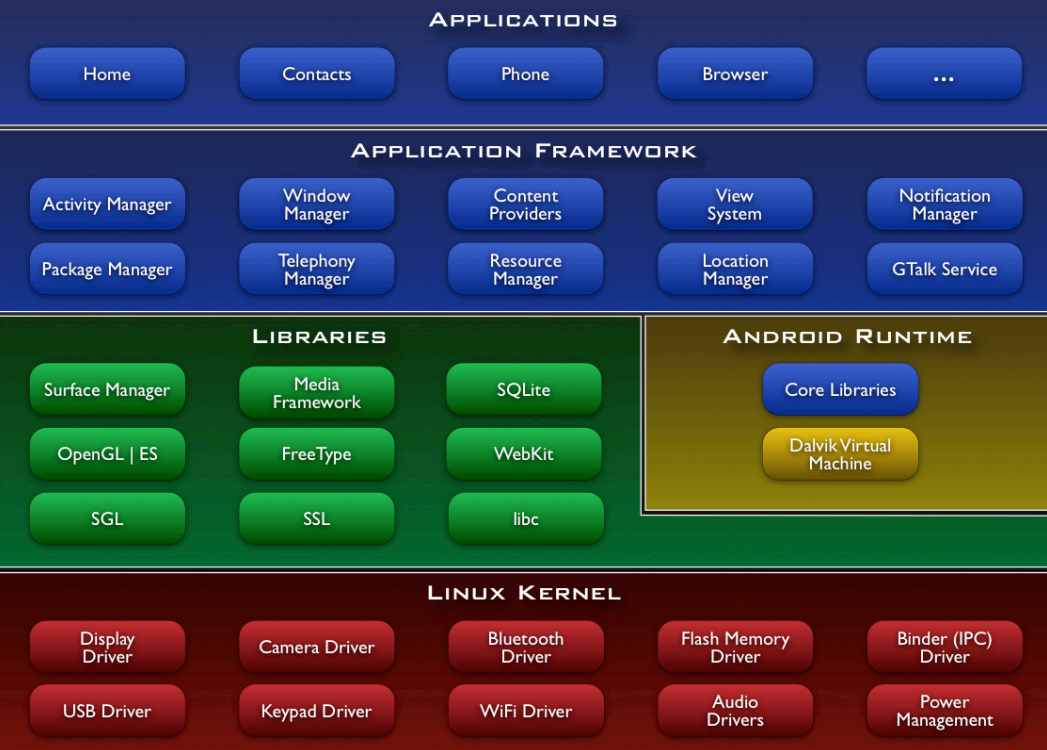
\includegraphics[width=0.825\textwidth]{AndroidArchitecture}
\caption{Android Architektur\cite{1}}
\label{fig:AndroidArchitecture}
\end{figure*}
\\
Ein weiterer bedeutender Unterschied liegt darin, dass eine Dalvik VM klassische Java Bibliotheken nicht unterstuetzt, zum Beispiel \member{AWT} und \member{Swing}. Es werden eigene Bibliotheken verwendet, die Apache Harmony als Grundlage verwenden.
\\
\\
Ein wichtiger Bestandteil der \member{SDK} ist das Tool \member{dx}. Es sorgt dafuer, dass Java Binaerdaten in Dalvik Executables umgewandelt werden. Das heist es wandelt \member{.class} Dateien in \member{.dex} Dateien um. Bei dieser Umwandlung koennen auch mehrere \member{.class} Dateien zu einer \member{.dex} Datei zusammengefasst werden, beziehungsweise kann der Speicherbedarf, mithilfe von \member{.odex} Dateien optimiert werden. 
\\
\\
In Abbildung 3 ist ein solcher Vorgang beispielhaft dargestellt. Zuerst werden die \member{.java} Dateien in \member{.class} Dateien kompiliert. Nach dem Kompiliervorgang werden die Binaerdateien und die \member{.class} Dateien mithilfe des \member{dx} Tools zu eienr \member{.dex} Datei konvertiert. Mithilfe dieser Datei kann nun eine \member{.apk} Datei erstellt werden. Bei dieser handelt es sich um die Applikationsdatei mit der, der Endbenutzer die Anwendung auf seinem Mobiltelefon installiert.

\begin{figure*}
\centering
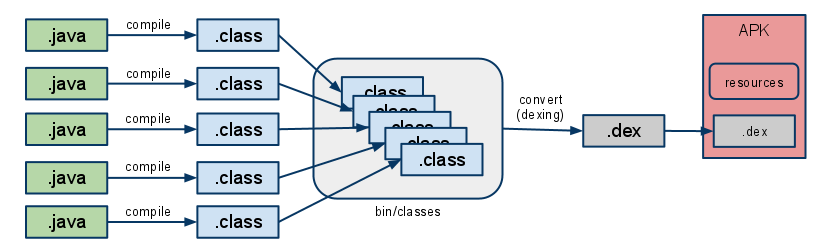
\includegraphics[width=\textwidth]{ClassToDex}
\caption{Android Kompiliervorgang\cite{7}}
\label{fig:ClassToDex}
\end{figure*}


\subsection{.dex Format}
In .dex Dateien werden die Klassen Definitionen und die dazugehoerigen Daten gespeichert. Es handelt sich dabei um die ausfuehrbaren Dateien der Dalvik VM. Android Programme werden zuerst in Java Bytecode kompiliert. Dieser wird im Anschluss in Dalvik Bytecode uebersetzt. 
\\
\\
In Abbildung 4 ist der Aufbau einer .dex Datei im Vergleich zu einer .class Datei von Java zu sehen. Fuer alle folgenden Listen der Datei duerfen keine doppelten Eintraege vorhanden sein.

\begin{figure}
\centering
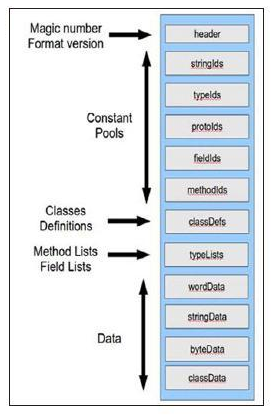
\includegraphics[width=0.4\textwidth]{DexFileFormat}
\caption{Dex Dateiformat\cite{1}}
\label{fig:DexFileFormat}
\end{figure}

\subsubsection{Header}
In Ausschnitt 1 ist der Header der \member{.dex} Datei zu sehen. Dabei handelt es sich um eine bestimmte Bytefolge die den Start der Datei bestimmt.

\begin{lstlisting}[float,floatplacement=H,caption=Dex Header\cite{2}]
ubyte[8] DEX_FILE_MAGIC = 
{ 0x64 0x65 0x78 0x0a 0x30 0x33 0x35 0x00 } 
= "dex\n035\0"

\end{lstlisting}

\subsubsection{StringIds}
Hierbei handelt es sich um eine Liste aller Strings die in der Datei verwendet werden. Die Liste muss sortiert sein und darf keine doppelten Eintraege enthalten. Moegliche Inhalte sind zum Beispiel konstante Strings und Funktionsnamen.

\subsubsection{TypeIds}
Dies ist eine Liste aller verwendeten Typen dieser Datei. Dazu gehoeren Klassen, Arrays, und Primitive Datentypen. Diese Liste ist nach den \member{StringIds} sortiert.

\subsubsection{ProtoIds}
In dieser Liste befinden sich alle Methoden Prototypen, die in \member{.dex} Datei verwendet werden. Die Prototypen sind primaer anhand ihrer Rueckgabetypen sortiert und danach anhand ihrer Argumente.

\subsubsection{FieldIds}
Diese Liste enthaelt alle Felder die von der \member{.dex} Datei referenziert werden. Diese Liste wird anhand des Feldtypen und Feldnamen sortiert.

\subsubsection{MethodIds}
In der Methoden Liste werden alle von der \member{.dex} Datei referenzierten Methoden aufgelistet. Diese Liste wird nach dem Methodennamen und dem Methodenprototypen sortiert.

\subsubsection{ClassDefs}
In dieser Liste werden die Klassendefinitionen der \member{.dex} Datei angegeben. Die Liste muss so geordnet werden, dass uebergeordnete Klassen und Interfaces vor den davon ableitenden Klassen angefuehrt werden.

\subsubsection{Data}
In dem Data werden zusaetzliche Daten fuer die oben angefuehrten Listen gespeichert. Die verschiedenen Elemente haben verschiedene Alignements und padding bytes werden, wenn notwendig, eingefuegt. Des weiteren befinden sich in diesem Bereich die Daten von statisch verlinkten Dateien. Bei nicht verlinkten Dateien ist dieser Teilbereich leer.


\subsection{Bytecode \& Instruction Format}
Das Modell der Dalvik VM ist an eine echte Architektur angelegt und soll Calling Conventions C ähnlich realisieren. 
Die Dalvik VM ist registerbasiert und ihre Frames bekommen bei der Erstellung eine fixe Größe zugewiesen. Jedes Frame besteht aus einer bestimmten Anzahl an Registern, die von einer Methode aus dem Bytecode Set vorgegeben wird. Zusätzlich beinhaltet das Frame noch alle zusätzlich benötigten Daten, so wie zum Beispiel Program Counter und die \member{.dex} Datei die die Methode beinhaltet.
Für Bitwerte, wie zum Beispiel \member{integer} und Gleitkommazahlen sind Register 32-Bit lang. Für 64-Bit Werte wird mit einem anliegenden Register ein Paar gebildet. Für Registerpaare wird kein Alignement benötigt. Wenn die Register für Objekt Referenzen benutzt werden, dann sind sie groß genug um exakt eine Referenz zu speichern. Bei einem Methodenaufruf werden N Argumente der Methode in den N letzten Registern des Frames der Methode platziert. Größere Argumente benötigen hierbei 2 Register. Methoden einer Instanz bekommen als ersten Parameter zusätzlich eine \member{this} Referenz übergeben.
\\
\\
Instruktionen sind nicht auf Datentypen limitiert, solange sie den Inhalt der Register nicht interpretieren. Ein Beispiel dafür ist der \member{move} Befehl, ihm ist es egal ob er \member{integer} oder \member{floats} verschiebt. Die meisten Instruktionen sind bei ihrer Ausführung auf die ersten 16 Register limitiert und können auf höhere Register nicht zugreifen. Wenn es möglich ist erlauben einige Instruktionen, aber auch Zugriff auf die ersten 256 Register. In einigen Ausnahmefällen wie zum Beispiel einzelnen \member{move} Instruktionen ist es möglich auf Register zwischen 0 und 65535 zuzugreifen.
Unterstützt eine Instruktion das gewünschte Register nicht muss das hohe Register vor der Operation in ein niederes Register kopiert und nach der Operation wieder zurück kopiert werden.
\\
\\
Die Dalvik VM besitzt einige Pseudoinstruktionen, die dazu verwendet werden um Daten mit variabler Länge zu verarbeiten zum Beispiel \member{fill-array-data}. Diese Instruktionen müssen auf 4 Byte aligned sein. Um dieses Ziel zu erreichen werden bei der Generierung der \member{.dex} Datei wenn nötig \member{nop} Instruktionen eingefügt. Wenn die Applikation auf einem System installiert wird können manche Instruktionen, aufgrund von Optimierungen, verändert werden. Damit kann eine schnellere Ausführung am System erreicht werden.
\\
\\
In Abbildung 5 sind einige Beispielinstruktionen der Dalvik VM zu sehen. Die Syntax ist so aufgebaut das zuerst das Ziel- und danach das Quellregister angegeben wird. Manche Opcodes haben Namenserweiterungen um gewisse Eigenschaften anzuzeigen. Zum Beispiel wird bei 64 Bit Opcodes \member{-wide} hinzugefügt und bei typenspezifischen Opcodes wird der Typ hinzugefügt, \member{-char}.
Anhand des \member{move-wide/from16 vAA, vBBBB} Opcodes lassen sich diese Eigenschaften gut erkennen. Der Opcode dieser Instruktion ist \member{move} daran lässt sich leicht erkennen das es sich um eine Operation zum verschieben von Registerwerten handelt. Das Attribut \member{wide} gibt an das die Instruktion auf 64-Bit lange Daten angewandt wird. Das Attribut \member{from16} gibt an das eine 16-Bit Register Referenz als Quelle dient. Die beiden Parameter \member{vAA} und \member{vBBBB} geben Quell- und Zielregister an. Wobei das Quellregister im Bereich \member{v0-v255} liegen muss und das Zielregister im Bereich \member{v0-v65535}.

\begin{figure*}
\centering
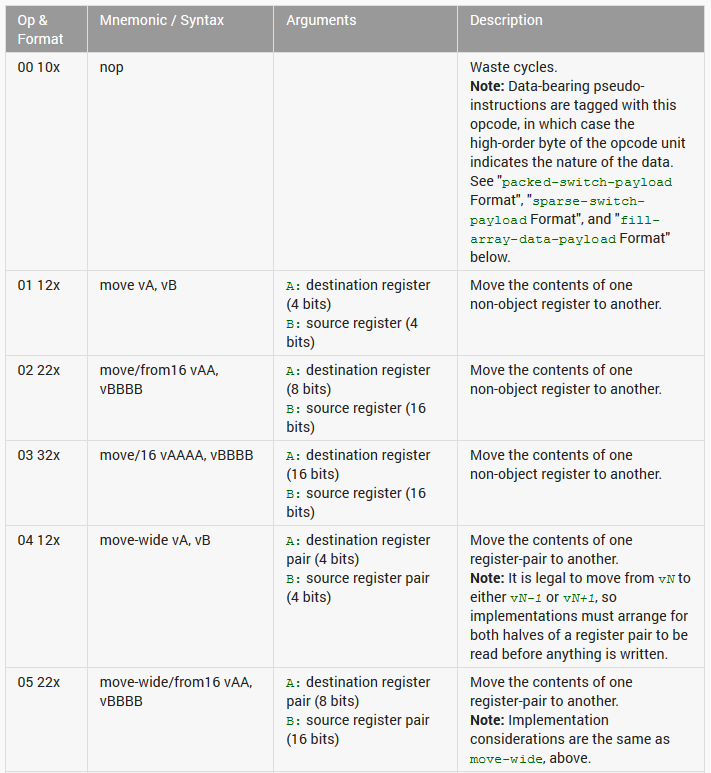
\includegraphics[width=0.6\textwidth]{ByteCode}
\caption{Dalvik VM Instruktionen\cite{2}}
\label{fig:ByteCode}
\end{figure*}


\section{Dalvik vs Android Runtime}
In diesem Kapitel wird die neuere Android Runtime näher betrachtet. Des weiteren wird die Dalvik VM mit der Android Runtime verglichen.

\subsection{Dalvik\cite{8}}
Dalvik ist ein Just-in-time-Compiler (JIT Compiler). Dabei werden Programme oder Programmteile zur Laufzeit in Maschinencode übersetzt. Da die Kompilierung während der Ausführung des Programms durchgeführt wird, kann sie nicht beliebig aufwendig sein, da dies sonst die Ausführungsgeschwindigkeit des eigentlichen Programms merklich beeinträchtigen könnte. Daher beschränkt man sich meist auf häufig ausgeführte Programmteile. Diese sind typischerweise für den Großteil der Ausführungszeit des Programms verantwortlich, weshalb sich deren Kompilation und Optimierung besonders lohnt.
\\
\\
Die Aufgabe des JIT-Compilers ist es, diese Programmteile zu identifizieren, zu optimieren und anschließend in Maschinencode zu übersetzen, welcher vom Prozessor direkt ausgeführt werden kann. Der erzeugte Code wird meist zwischengespeichert, um ihn zu einem späteren Zeitpunkt der Programmausführung wiederverwenden zu können.

\subsection{Android Runtime\cite{4}}
Android Runtime (kurz ART) ist eine Laufzeitumgebung die von Googles mobilem Betriebssystem Android ab Version 5.0 Lollipop eingesetzt wird.
ART löste damit die bisherige virtuelle Maschine Dalvik ab, die bis Version 4.4 (KitKat) im Einsatz war. Laut Google bietet ART eine bessere Performance und niedrigen Energieverbrauch als Dalvik. Dies wird sich in der Praxis in besserer Performance und längerer Akkulaufzeit bemerkbar machen.

\subsection{Vergleich\cite{9}}
Bei Android Runtime handelt es sich um einen Ahead-of-time-Compiler (AOT-Compiler). Ein AOT-Compiler ist ein Compiler, der im Gegensatz zu Just-in-time-Compilern (JIT-Compiler) Programmcode vor der Ausführung in native Maschinensprache übersetzt. Dies hat den Vorteil, dass dieser Code zur Laufzeit wesentlich schneller ausgeführt wird als auf einem JIT-Compiler, da die Übersetzung bereits durchgeführt wurde. Dabei wird der Java-Bytecode bereits bei der Installation einer App in maschinenlesbaren Code vorkompoliert. 
\\
\\
Der Nachteil an AOT-Compilern ist aber, dass dieser Code nicht mehr plattformunabhängig ist, wie es bei JIT-Compilern der Fall ist. AOT-Compiler sind die herkömmlichen Compiler wie sie schon von C eingesetzt wurden. Da Bytecode prinzipiell speichermäßig kleiner als Maschinencode ist, kann die Größe einer installierten App schnell auf bis zu zusätzlich 20\% ansteigen. Außerdem dauert die Installation einer App länger als zuvor, da der Bytecode bereits hier in Maschinencode übersetzt wird.
\\
\\
ART liefert Untersuchungen zufolge, in vielen Apps mehr Leistung als Dalvik. Grund ist, dass der Bytecode durch ART erheblich maschinennäher als Dalvik formuliert wird und somit weniger Rechenaufwand zur Ausführung vonnöten ist. Dies bedeutet, dass die Ressourcen des Geräts effizienter genutzt werden können und die gefühlte Performance ansteigt.
\\
\begin{figure*}
\centering
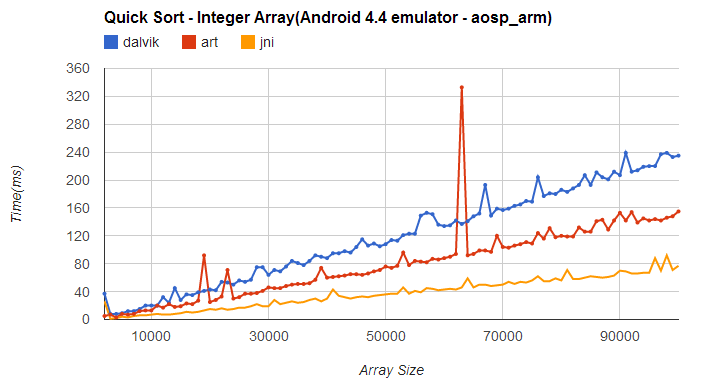
\includegraphics[width=1\textwidth]{DalvikVMARTVergleich}
\caption{Dalvik VM ART Vergleich\cite{10}}
\label{fig:DalvikVMARTVergleich}
\end{figure*}
\\
ART und Dalvik sind kompatiblel zueinander, das bedeutet Apps, die für Dalvik implementiert wurden, laufen auch auf ART. Die ART benutzt dabei denselben Input Bytecode wie Dalvik, geliefert mit Standard .dex-Dateien als Teil der Android Application Package-Dateien (APK-Dateien), wobei die .odex-Dateien durch Executable and Linkable Format (ELF) – Executables ersetzt werden. Da die Kompilierung nicht bei jeder Ausführung einer Applikation durchgeführt werden muss, wird die Prozessorauslastung verringert und dadurch die Akkulaufzeit verbessert.


\subsection{Neuheiten in Android Runtime\cite{11}\cite{12}}

\subsubsection{Verbesserte Garbage Collection}
GC kann die Performance einer App beeinflussen, also abgehackte Bilder, langsame Reaktion auf Benutzerinteraktionen oder andere Probleme. Verbesserungen sind unter anderem, dass weniger Ausführungen des Garbace Collector’s gemacht werde und während der GC-Pause trotzdem Anwendungen parallel laufen können. Außerdem wird der GC kürzer ausgeführt für kurzlebige Objekte.

\subsubsection{Verbesserungen für Entwicklung und Debugging}
Für Dalvik wurde das Tool Traceview als Profiler verwendet, also zur Analyse des Laufzeitverhaltens von Software. Dieses gibt zwar sinnvolle Informationen, jedoch wird bei jedem Aufruf durch das Tool der Overhead größer, wodurch die Laufzeit beeinflusst wird.
Bei Traceview verwendet die Debug class um Informationen im Code zu protokollieren. Die log-Dateien können geladen werden und in 2 unterschiedlichen Panels angezeigt werden:
\\
\\
Timeline Panel (Abbildung 7): zeigt wann jeder Thread und jede Methode startet und stoppt.
\\
\begin{figure*}
\centering
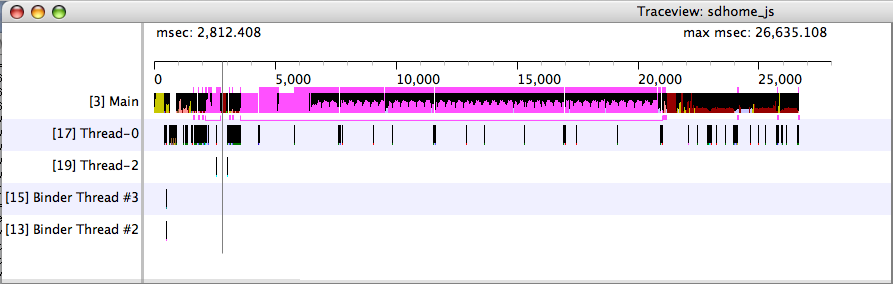
\includegraphics[width=1\textwidth]{traceviewTimeline}
\caption{Traceview Timeline\cite{12}}
\label{fig:traceviewTimeline}
\end{figure*}
\\
Profile Panel (Abbildung 8): stellt einen Überblick dar von Ereignissen innerhalb der Methoden.
\\
\begin{figure*}
\centering
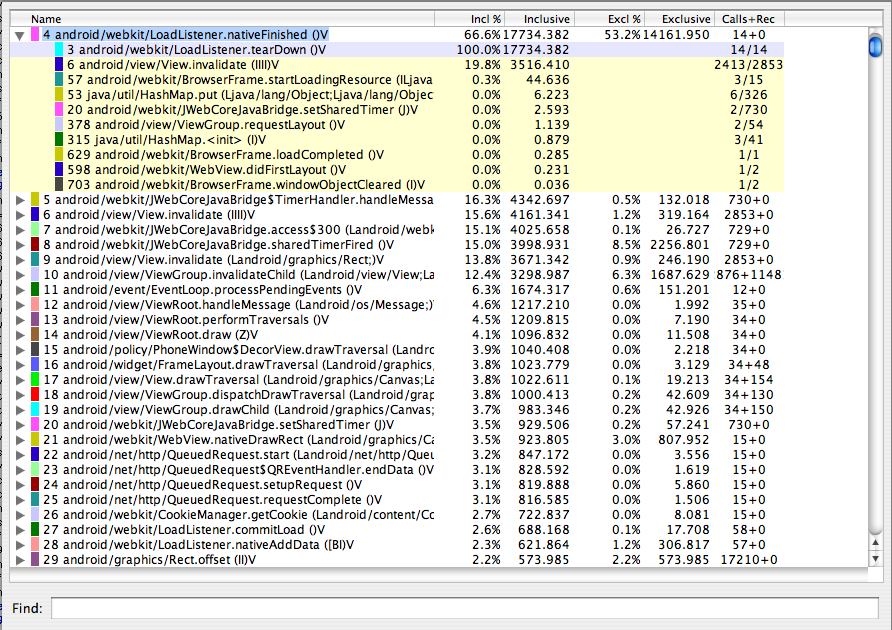
\includegraphics[width=1\textwidth]{traceviewProfile}
\caption{Traceview Profile\cite{12}}
\label{fig:traceviewProfile}
\end{figure*}
\\
ART unterstützt einen geeigneten Profiler der diese Einschränkungen nicht hat. Dadurch gibt es eine detaillierte Sicht über die Ausführung der App ohne eine erhebliche Verlangsamung.

\subsubsection{Mehr Debugging Features}
Man kann anzeigen welche Locks im Stack gehalten werden und zu dem Thread springen, der den Lock hält. Es ist außerdem möglich nachzusehen, wie viele Instanzen einer Klasse existieren und welche Referenzen diese haben. Zusätzlich gibt es sogenannte „method-exit“-events, die anzeigen, welche Werte bestimmte Methoden zurückliefern, und man kann „Watchpoints“ auf Members setzen und die Ausführung unterbrechen falls auf diese zugegriffen wird bzw. diese modifiziert werden.

\subsubsection{Verbesserte Diagnose in Exceptions und Crash Reports}
ART gibt so viele Details wie möglich falls Exceptions zur Laufzeit auftreten. Zum Beispiel zeigt die java.lang.NullpointerException Informationen darüber was die App mit dem Nullpointer versuchte zu tun, wie auf einen Wert zu schreiben oder der Versuch, eine Methode aufzurufen. Ein Beispiel dazu ist in Ausschnitt 2 zu sehen.

\begin{lstlisting}[float,floatplacement=H,caption=Exception]
java.lang.NullPointerException: Attempt to 
write to field 'int android.
accessibilityservice.AccessibilityService
Info.flags' on a null object reference

java.lang.NullPointerException: Attempt to 
invoke virtual method 'java.lang.String 
java.lang.Object.toString()' on a null 
object reference
\end{lstlisting}


\bibliographystyle{IEEEtran}

\bibliography{IEEEexample}

\end{document}
